% !TeX program = lualatex
% !TeX encoding = utf8
% !TeX spellcheck = uk_UA
% !BIB program = bibler

\documentclass[onlytextwidth]{beamer}
\usetheme{Electromagnetism}
\usepackage{Electromagnetism}
\usepackage{circuitikz}


%============================================================================
\title[Лекції електрики та магнетизму]{\huge\bfseries Явище електромагнітної індукції}
\subtitle{Лекції з електрики та магнетизму}
\author{Пономаренко С. М.}
\date{}
%============================================================================
\graphicspath{{pictures/}}
\begin{document}
\begin{frame}[plain]
	\maketitle
\end{frame}

% ============================== Слайд ## ===================================
\begin{frame}{Зміст}{}
	\tableofcontents
\end{frame}
% ===========================================================================



%% --------------------------------------------------------
\section{Явище електромагнітної індукції}
%% --------------------------------------------------------



% ============================== Слайд ## ===================================
\begin{frame}{Явище електромагнітної індукції}{}
	\begin{block}{Явище електромагнітної індукції (Фарадей)}\justifying
		У 1831 р. Фарадеєм було зроблено одне з найбільш фундаментальних відкриттів в електродинаміці --- \alert{явище електромагнітної індукції}. Воно
		полягає в тому, що в замкненому провідному контурі при зміні магнітного потоку, охопленого цим контуром, виникає електричний струм --- його назвали
		індукційним.
	\end{block}

	\vfill

	\href{https://youtu.be/GrBYG8NIUoU}{\color{blue}\small Досліди Фарадея}

\end{frame}
% ===========================================================================



% ============================== Слайд ## ===================================
\begin{frame}{Закон електромагнітної індукції}{}
	\begin{block}{}\justifying
		Електрорішійна сила (ЕРС), що виникає в контурі пропорційна швидкості зміни магнітного потоку, що пронизує площу, охоплену даним контуро:
		\begin{equation*}
			\tcbhighmath{\mathcal{E}_\text{ind} =  -\frac1c \frac{d\Phi}{dt}} = -\frac1c \frac{d}{dt} \iint\limits_S.
		\end{equation*}
	\end{block}
	\begin{columns}
		\begin{column}{0.5\linewidth}\centering
			\begin{tikzpicture}[rotate=90, scale=0.9, >=latex, midarrow/.style={%
							postaction={ decorate,
									decoration={ markings, mark=at position .7 with {\arrow{latex}}}}}]
				\begin{scope}%[rotate around={45:(0,1)}]
					\draw[arrowpos={0.5}{2pt}{7pt}, red!40, ultra thick] (1.1,0) [partial ellipse=360:0:0.3 and 1];
				\end{scope}

				\foreach \y in {-3,...,3}{
						\draw[blue, midarrow] plot[domain=1:3] (\x, 0.2*\y+0.05*\y*\x^2);
					}
				\node[blue, font=\small] at (3.5, 0) {$\frac{d\Phi}{dt}>0$};
			\end{tikzpicture}
		\end{column}
		\begin{column}{0.5\linewidth}\centering
			\begin{tikzpicture}[rotate=90, scale=0.9, >=latex, midarrow/.style={%
							postaction={ decorate,
									decoration={ markings, mark=at position .7 with {\arrow{latex}}}}}]
				\begin{scope}%[rotate around={45:(0,1)}]
					\draw[arrowpos={0.5}{2pt}{7pt}, red!40, ultra thick] (1.1,0) [partial ellipse=0:360:0.3 and 1];
				\end{scope}

				\foreach \y in {-3,...,3}{
						\draw[blue, midarrow] plot[domain=1:3] (\x, 0.2*\y+0.05*\y*\x^2);
					}
				\node[blue, font=\small] at (3.5, 0) {$\frac{d\Phi}{dt}<0$};
			\end{tikzpicture}
		\end{column}
	\end{columns}
	\begin{block}{Правило Ленца}\justifying\small
		Індукований струм має такий напрямок, щоб за допомогою
		створюваного ним магнітного поля перешкоджати зміні
		магнітного потоку, тобто щоб послабити дію причини, яка збуджує
		цей струм.
	\end{block}
\end{frame}
% ===========================================================================


% ============================== Слайд ## ===================================
\begin{frame}{Струми Фуко}{}
	\begin{block}{}\justifying
		Струми Фуко --- вихрові індукційні струми, які виникають у провіднику під час зміни магнітного потоку через поверхню провідника.
	\end{block}
	\begin{center}
		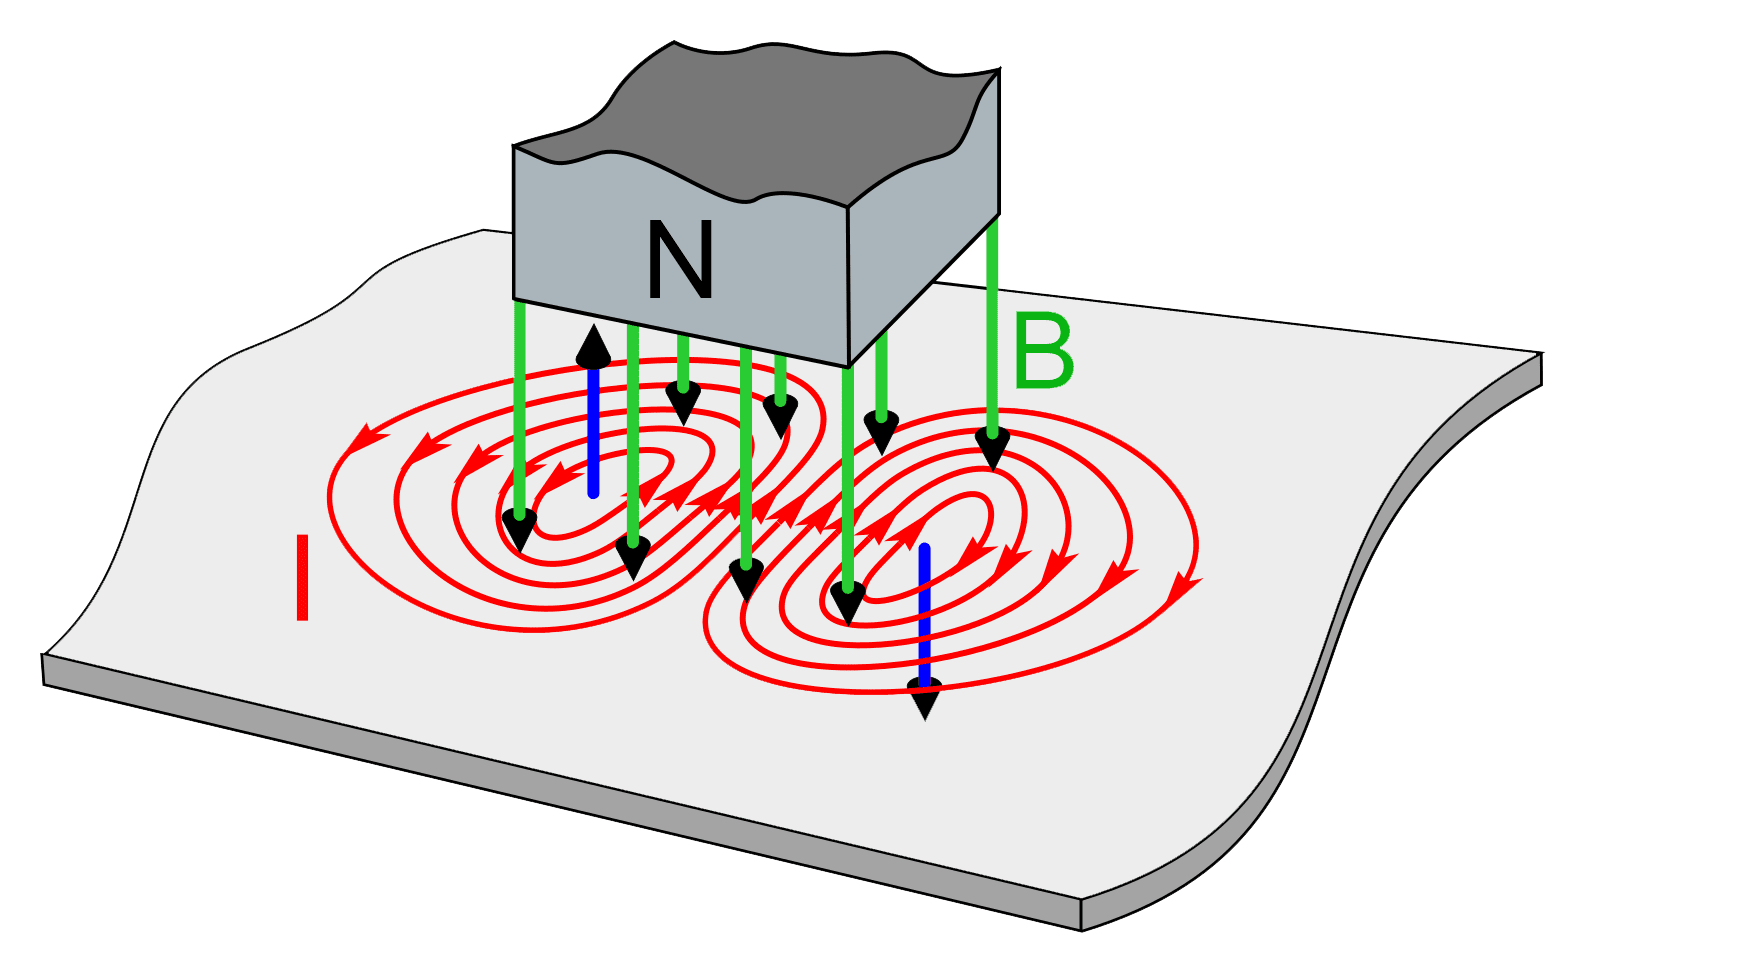
\includegraphics[width=.5\linewidth]{Fuko_currents}
	\end{center}

	\begin{block}{}\justifying
		Струми Фуко, як і індукційні струми в лінійних провідниках, підпорядковані правилу Ленца: їх магнітне поле направлене так, щоб протидіяти змінам
		магнітного потоку, що індукували ці струми.
	\end{block}
\end{frame}
% ===========================================================================


% ============================== Слайд ## ===================================
%\begin{frame}{Закон збереження магнітного потока}{}
%
%\end{frame}
% ===========================================================================




%% --------------------------------------------------------
\subsection{Вихрове електричне поле}
%% --------------------------------------------------------



% ============================== Слайд ## ===================================
\begin{frame}{Вихрове електричне поле}{}
	\begin{onlyenv}<1>
		\begin{block}{}\justifying
			Оскільки магнітний потік дорівнює $\Phi = \iint\limits_S \Bfield\cdot d\vect{S}$, а ЕРС індукції $\mathcal{E} = \oint\limits_L \vect{E}\cdot
				d\vect{\ell}$,
			то із закону індукції  випливає:
			\begin{equation*}
				\oint\limits_L \Efield\cdot d\vect{\ell} = \iint\limits_S \Bfield\cdot d\vect{S}.
			\end{equation*}
			Скориставшись теоремою Стокса, останнє інтегральне рівняння можна переписати у диференціальній формі:
		\end{block}
	\end{onlyenv}
	\begin{onlyenv}<1-2>
		\begin{block}{}\justifying
			\begin{equation*}
				\tcbhighmath{\Rot\Efield = - \frac1c \frac{\partial\Bfield}{\partial t}.}
			\end{equation*}
		\end{block}
	\end{onlyenv}
	\begin{onlyenv}<2>
		\begin{columns}
			\begin{column}{0.4\linewidth}\centering
				\begin{tikzpicture}[rotate=90, scale=0.9, >=latex, midarrow/.style={%
								postaction={ decorate,
										decoration={ markings, mark=at position .7 with {\arrow{latex}}}}}]
					\begin{scope}%[rotate around={45:(0,1)}]
						\draw[arrowpos={0.5}{2pt}{4pt}, red] (1.1,0) [partial ellipse=360:0:0.15 and 0.5];
						\draw[arrowpos={0.5}{2pt}{4pt}, red] (1.1,0) [partial ellipse=360:0:0.3 and 1];
						\draw[arrowpos={0.5}{2pt}{4pt}, red] (1.1,0) [partial ellipse=360:0:0.6 and 2] node[pos=0.5, below] {$\Efield$};
					\end{scope}

					\foreach \y in {-3,...,3}{
							\draw[blue, midarrow] plot[domain=1:3] (\x, 0.2*\y+0.05*\y*\x^2);
						}
					\node[blue, font=\small] at (3.5, 0) {$\frac{\partial\Bfield}{\partial t}>0$};
				\end{tikzpicture}
			\end{column}
			\begin{column}{0.6\linewidth}
				\begin{block}{}\justifying\small
					Згідно  Максвеллу \alert{явище електромагнітної індукції} полягає в тому, що будь-яке змінне магнітне поле збуджує в просторі
					електричне поле; провідники для цього не потрібні. Індукційні ж струми збуджуються в провідниках індукованим електричним полем.
				\end{block}
			\end{column}
		\end{columns}
		\begin{block}{}\justifying\small
			На відміну від електростатики, де $\Rot\Efield = 0$, у випадку змінного в чаі магнітного поля $ \Rot\Efield \neq 0$. Це означає, що
			індуковане
			електричне поле, індукується (виникає) за рахунок зміни магнітного поля і не є потенційним, а вихровим.
		\end{block}
	\end{onlyenv}
\end{frame}
% ===========================================================================


% ============================== Слайд ## ===================================
\begin{frame}{Вираз електричного поля через потенціали}{}
	\begin{block}{}
		Скористаємося законом електромагнічної індукції. Підставимо
		сюди вираз для магнітного поля через векторний потенціал
		\(
		\Bfield=\Rot\vect{A}
		\):
		\begin{equation*}
			\Rot\left(\Efield  + \frac{\partial\vect{A}}{\partial t}\right) = 0
		\end{equation*}
		Рівність нулю ротора деякого векторного поля означає, що це
		поле потенційне і може бути представлене як градієнт скалярної
		функції. Таким чином, отримуємо
		\begin{equation*}
			\Efield = -\vect{\nabla}\phi - \frac{\partial\vect{A}}{\partial t}
		\end{equation*}
		У окремому випадку постійних у часі полів приходимо до відомої
		рівності: $\Efield = -\vect{\nabla}\phi $, звідки видно, що введена тут функція $\phi$
		збігається зі скалярним потенціалом.
	\end{block}
\end{frame}
% ===========================================================================



%% --------------------------------------------------------
\section{Явище самоіндукції}
%% --------------------------------------------------------



% ============================== Слайд ## ===================================
\begin{frame}{Явище самоіндукції}{}
	\begin{block}{}\justifying
        Зміна струму в контурі викликає зміну магнітного поля, що створює змінний магнітний потік через цей же контур і, як наслідок, ЕРС індукції. Це
        явище називають \alert{самоіндукцією}.
	\end{block}
	\begin{columns}
		\begin{column}{0.35\linewidth}\centering
			\begin{tikzpicture}[rotate=90, scale=0.9, >=latex, midarrow/.style={%
							postaction={ decorate,
									decoration={ markings, mark=at position .7 with {\arrow{latex}}}}}]
				\begin{scope}%[rotate around={45:(0,1)}]
					\draw[arrowpos={0.5}{2pt}{7pt}, red!40, ultra thick] (1.1,0) [partial ellipse=0:360:0.3 and 1] node[pos=0.5, below] {$I$};
				\end{scope}
				\foreach \y in {-3,...,3}{
						\draw[blue, midarrow] plot[domain=1:3] (\x, 0.2*\y+0.05*\y*\x^2);
					}
			\end{tikzpicture}
		\end{column}
		\begin{column}{0.65\linewidth}
            \begin{onlyenv}<1>
    			\begin{block}{}\justifying
    				Якщо в просторі, де розташований контур зі
    				струмом $I$, немає феромагнетиків, поле $\Bfield$, а отже, і повний
    				магнітний потік $\Phi$ через контур будуть пропорційні силі
    				струму $I$:
    				\begin{equation*}
    					\Phi = \frac1c L I
    				\end{equation*}
    			\end{block}
            \end{onlyenv}
            \begin{onlyenv}<2>
    			\begin{block}{}\justifying
                    При зміні сили струму в контурі згідно закону Фарадея виникає ЕРС самоіндукції:
                    \begin{equation*}
                        \mathcal{E} = - L\frac{dI}{dt}
                    \end{equation*}
                      {\scriptsize Тут знак мінус показує, що $\mathcal{E}$ завжди спрямована так, щоб перешкоджати зміні сили струму відповідно до
                      правила Ленца. Ця ЕРС прагне зберегти струм незмінним: вона протидіє струму, коли він збільшується, і підтримує струм, коли він
                      зменшується.}
    			\end{block}
            \end{onlyenv}
		\end{column}
	\end{columns}
\begin{block}{}
Коефіцієнт $L$ називається \alert{індуктивністю контуру}.
\end{block}
\end{frame}
% ===========================================================================


% ============================== Слайд ## ===================================
\begin{frame}{Приклади розрахунку індуктивності}{}

\end{frame}
% ===========================================================================

\end{document}
